% Double-anonymous ICSEC 2026 review manuscript.
\documentclass[conference]{IEEEtran}
\usepackage[T1]{fontenc}
\usepackage{newtxtext,newtxmath}
\usepackage{graphicx}
\usepackage{booktabs}
\usepackage{amsmath}
\usepackage{cite}
\usepackage{algorithm}
\usepackage{algpseudocode}
\usepackage[hidelinks,pdftitle={Cross-Platform Profile Identity Resolution for an Agentic CRM Platform Using Genetic Optimization of Three-Way Decisions},pdfauthor={Anonymous},pdfsubject={Double-anonymous ICSEC 2026 review manuscript},pdfkeywords={entity resolution, record linkage, cross-platform identity linkage, genetic algorithm, three-way decision}]{hyperref}
\newcommand{\pmv}{\,$\pm$\,}
\begin{document}

\title{Cross-Platform Profile Identity Resolution for an Agentic CRM Platform Using Genetic Optimization of Three-Way Decisions}
\author{\IEEEauthorblockN{Anonymous Submission}}
\maketitle

\begin{abstract}
Agentic customer-relationship-management (CRM) systems require consolidated identities before automated components can use fragmented profile information. Cross-platform identity resolution addresses this prerequisite by deciding whether incomplete profiles from different services refer to the same individual. A pair classifier can estimate matching evidence, but a score alone does not determine whether a workflow should merge, defer, or reject a pair. We evaluate a three-way policy that converts isotonic-calibrated Gradient Boosting scores into MATCH, REVIEW, or NO\_MATCH. A Genetic Algorithm (GA) selects four policy parameters using validation entities without retraining the classifier. Experiments on a transformed LinkSocial derivative use three repeated outer evaluations in which classifier training, calibration, GA selection, and sealed testing have disjoint entities. The GA policy attains mean F1 $0.8604$ versus $0.8280$ for fixed thresholds and raises mean recall from $0.7100$ to $0.7615$. This is an operating trade-off: mean precision decreases from $0.9940$ to $0.9889$, false positives increase from $38.0$ to $75.7$, and REVIEW decisions from $438.0$ to $923.3$. Candidate generation reduces 449,149,239 possible cross-platform comparisons to 2,086,245 workflow candidates, but covers only 25,931 of 29,243 positive pairs (88.6742\% retrieval recall). Thus, 3,312 true pairs never reach downstream scoring. Evidence is limited to one historical corpus; downstream CRM agents, lead scoring, human review, and business outcomes are not evaluated.
\end{abstract}

\begin{IEEEkeywords}
entity resolution, record linkage, cross-platform identity linkage, genetic algorithm, three-way decision, probability calibration
\end{IEEEkeywords}

\section{Introduction}
An Agentic CRM system may coordinate retrieval, recommendation, communication, and other automated activities around a customer record. Those activities first require a defensible identity layer: observations from different channels must be associated with the correct person. Incorrect consolidation can propagate unrelated evidence into one record, while fragmented identities prevent a system from using information already available elsewhere. This paper treats Agentic CRM only as the application context and evaluates the upstream identity-resolution component, not CRM agents, lead scoring, or business outcomes.

Cross-platform profile identity resolution asks whether accounts observed on different services belong to the same individual. Consider a profile $A$ on platform $X$ and profile $B$ on platform $Y$. Their usernames may differ, one biography may be incomplete, their URLs may use different domains, and location may be missing; nevertheless, the profiles may describe the same person. Conversely, similar display names do not establish identity. The problem therefore requires combining several weak and sometimes unavailable evidence sources \cite{shu2017uilreview,yao2023profile}.

A conventional learning pipeline first generates plausible candidate pairs, constructs pairwise similarities, and applies a classifier that outputs a match score. Candidate generation is essential because comparing every cross-platform pair grows quadratically \cite{papadakis2021blocking,li2020blocking}. The classifier can combine lexical similarities, profile attributes, missingness indicators, and semantic text representations; modern entity-matching work similarly studies learned and transformer-based representations \cite{barlaug2021survey,li2020ditto}.

A classification score is not yet an operational action. A high-confidence pair may be accepted as MATCH, an ambiguous pair may be routed to REVIEW, and an implausible pair should remain NO\_MATCH. These outcomes have asymmetric consequences: a false merge combines different people, a false negative leaves one person fragmented, and REVIEW consumes scarce attention. Reject-option classification and human-in-the-loop ER therefore motivate evaluating coverage and review burden together with classification quality \cite{hendrickx2024reject,qian2019systemer}.

Three-way record linkage already exists \cite{ouyang2019threeway}, and genetic algorithms have already been applied to ER \cite{sun2017gaer}. We claim neither concept as new. The narrower question is: \emph{Can validation-selected genetic optimization alter the operational trade-off of fixed calibrated profile-matching probabilities under leakage-safe entity-disjoint evaluation?} The classifier and calibrator are frozen before policy optimization so that any subsequent change can be attributed to the decision layer.

We study three research questions. \emph{RQ1}: Does adding one MiniLM semantic-similarity feature improve a fixed-threshold Gradient Boosting workflow consistently? \emph{RQ2}: Relative to fixed thresholds, how does a GA-selected three-way policy change precision, recall, F1, false positives (FP), false negatives (FN), REVIEW volume, and a declared scenario-specific decision objective? \emph{RQ3}: How strongly does candidate retrieval constrain attainable end-to-end recall?

The contributions are: (1) a reproducible four-role protocol separating classifier training, probability calibration, policy selection, and sealed testing by entity; (2) controlled GB-17/GB-18 and GB-18/GB-18-GA comparisons that isolate representation and policy effects; (3) repeated outer-split evidence exposing both the GA policy's recall/F1 gain and its FP/REVIEW trade-off; and (4) a retrieval-to-decision decomposition that prevents pair-scoring improvements from being presented as complete workflow gains.

\section{Related Work}
\subsection{Cross-Platform Identity Resolution}
User identity linkage combines profile, content, and network evidence across services \cite{shu2017uilreview}. Profile methods use names, biographies, URLs, and other semi-structured attributes \cite{yao2023profile}; network structure can supplement attributes when available \cite{shu2017uilreview}. LinkSocial supplies the three-platform corpus used here \cite{linkSocial2018}. We evaluate profile evidence because the local derivative lacks a comparable current social graph.

\subsection{Candidate Generation and Pair Representation}
Blocking restricts comparison to likely pairs, trading computation for completeness \cite{papadakis2021blocking,li2020blocking}; a classifier cannot recover a true pair that blocking excludes. Learned blocking can retrieve candidates from semantic representations \cite{thirumuruganathan2021deepblocker}, whereas this study audits a fixed lexical/domain scheme and does not propose improved blocking. Pre-trained language models can encode heterogeneous records \cite{li2020ditto}. Because neural methods target different pipeline stages \cite{barlaug2021survey}, we report the retrieval ceiling separately and treat MiniLM cosine as one controlled feature, not a new semantic matcher.

\subsection{Three-Way and Human-Review Decisions}
Classical linkage formalizes probabilistic match decisions \cite{fellegi1969theory}; reject-option theory formalizes the error--rejection trade-off \cite{chow1970reject}. Three-way linkage adds a deferred region \cite{ouyang2019threeway}. Human-in-the-loop ER systems combine model decisions with analyst interaction \cite{qian2019systemer}. Here REVIEW is only an offline category; analyst effort, agreement, accuracy, and productivity are not measured.

\subsection{Evolutionary Optimization and Evaluation}
GA-based ER with active learning is prior art \cite{sun2017gaer}. Our GA instead tunes a downstream policy over persisted probabilities. Isotonic regression provides the probability-like scale used by that policy \cite{niculescu2005calibration}. Pair-random evaluation can place one entity in different experimental roles; entity-level assignment prevents this dependency leakage. We report multiple outcomes because linkage rankings can depend on the application error regime \cite{christen2026consistent}.

\section{System Overview}
Figure~\ref{fig:system} summarizes the decision path. Candidate generation retains cross-platform pairs sharing an exact or blocking key. Pair representation combines lexical, attribute, availability, and optional semantic evidence. Gradient Boosting produces a score, isotonic regression maps it to $p$, and a fixed or GA-selected policy emits MATCH, REVIEW, or NO\_MATCH. The evaluation ends at pair decisions; downstream CRM behavior is not tested.

\begin{figure*}[t]
\centering
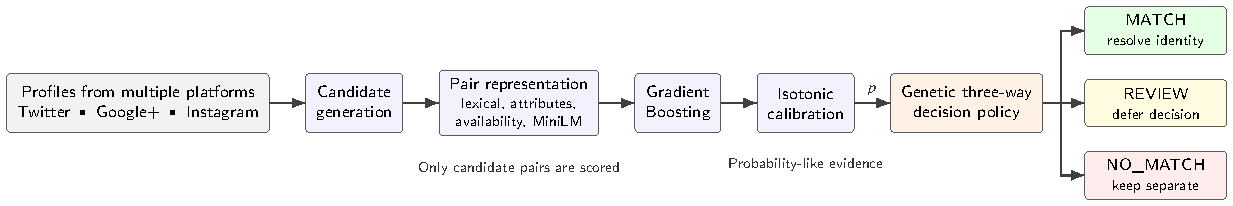
\includegraphics[width=\textwidth]{figures/system_overview.pdf}
\caption{Cross-platform identity resolution pipeline. Candidate generation limits which pairs reach scoring; the decision policy converts calibrated evidence into an operational outcome.}
\label{fig:system}
\end{figure*}

\section{Methodology}
\subsection{Dataset, Labels, and Candidate Generation}
Experiments use a locally transformed derivative of LinkSocial \cite{linkSocial2018}. Candidate generation requires valid profile and row identifiers, leaving 36,804 eligible profiles: Twitter (13,959), Google+ (11,889), and Instagram (10,956). Two profiles receive a positive label when they share the same non-empty source entity identifier. This yields 29,247 all-platform positive pairs, of which four are same-platform and excluded; the paper's cross-platform retrieval denominator is therefore 29,243. The public repository documents basic profile fields, but no machine-readable reuse license or formal ethics record was found; raw records are not redistributed.

The exact tier groups cross-platform profiles by normalized username or cleaned external URL. Remaining candidates share at least one of three keys: the first three normalized username characters, the first three normalized full-name characters, or a non-generic external domain. Table~\ref{tab:retrieval} shows that the workflow retains 2,086,245 pairs from 449,149,239 possible cross-platform comparisons. This reduction makes scoring tractable but omits 3,312 true cross-platform pairs.

\begin{table}[t]
\caption{Cross-platform candidate decomposition.}
\label{tab:retrieval}
\centering
\begin{tabular}{@{}lr@{}}
\toprule
Measure & Value\\
\midrule
Eligible profiles (T / G+ / I) & 13,959 / 11,889 / 10,956\\
All / cross-platform positive pairs & 29,247 / 29,243\\
Same-platform positives excluded & 4\\
Possible cross-platform pairs & 449,149,239\\
Exact-tier / model-scored pairs & 12,403 / 2,073,842\\
Total workflow candidates & 2,086,245\\
Covered positives / blocking misses & 25,931 / 3,312\\
Space reduction / retrieval recall & 99.5355\% / 88.6742\%\\
\bottomrule
\end{tabular}
\end{table}

\subsection{Pair Representation and Classification}
The handcrafted GB-17 representation contains 17 features: Jaro--Winkler, normalized Levenshtein, and token-order similarities for usernames and full names; maximum cross-field name similarity; biography token Jaccard, length ratio, and availability; location fuzzy, exact, and availability indicators; and platform agreement, username-length difference, full-name word-count difference, and username-prefix agreement. Same-platform is zero in this cross-platform scope but retained to preserve the frozen representation.

GB-18 adds only \texttt{bert\_cos}, cosine similarity between normalized \texttt{all-MiniLM-L6-v2} embeddings of concatenated full name, biography, and location. GB-17 and GB-18 use identical sampled training pairs, labels, seed, and settings: \texttt{GradientBoostingClassifier} with 300 estimators, learning rate 0.05, maximum depth 6, and seed 42. Training negatives are deterministically undersampled to 3:1.

\subsection{Calibration and Fixed Policy}
A separate isotonic regressor is fitted for each classifier using calibration entities only, with out-of-range predictions clipped. Calibration is not used to claim probabilistic correctness; it provides a monotone probability-like scale for the downstream policy. The fixed baseline applies MATCH when $p\geq0.98$, REVIEW when $0.95\leq p<0.98$, and NO\_MATCH otherwise.

\subsection{Genetic Three-Way Decision Policy}
Let $p$ be calibrated GB-18 probability and let $n$ be the maximum Jaro--Winkler similarity across username/full-name field combinations. A genome
\begin{equation}
 g=[t_{match},t_{review},c_{promote},c_{demote}]
\end{equation}
controls the policy in Algorithm~\ref{alg:policy}. The two $t$ genes delimit the probability regions. Within the intermediate region, $c_{promote}$ allows strong name evidence to promote a pair to MATCH, while $c_{demote}$ sends weak name evidence to NO\_MATCH; remaining pairs become REVIEW. Bounds are $0.90\leq t_{match}\leq0.999$, $0.50\leq t_{review}\leq t_{match}$, $0.50\leq c_{promote}\leq1$, and $0\leq c_{demote}\leq c_{promote}$.

\begin{algorithm}[t]
\caption{Three-Way Decision Policy}
\label{alg:policy}
\begin{algorithmic}[1]
\Require calibrated probability $p$, name evidence $n$, genome $g$
\Ensure MATCH, REVIEW, or NO\_MATCH
\If{$p \ge t_{match}$}
  \State \Return MATCH
\ElsIf{$p \ge t_{review}$}
  \If{$n \ge c_{promote}$} \State \Return MATCH
  \ElsIf{$n < c_{demote}$} \State \Return NO\_MATCH
  \Else \State \Return REVIEW
  \EndIf
\Else
  \State \Return NO\_MATCH
\EndIf
\end{algorithmic}
\end{algorithm}

The GA evaluates seeds $\{7,42,123,999,2025\}$. Each run uses population 60, 40 generations, 12 elites, uniform crossover, and per-gene Gaussian mutation with probability 0.30 and standard deviation 0.02. The selected run has the smallest validation objective, with the smaller seed breaking ties. Selection minimizes
\begin{equation}
U=2\,FP+FN+0.1\,REVIEW.
\end{equation}
This illustrative operational utility encodes engineering assumptions: false merges receive twice the penalty of missed matches, while review has a smaller, non-zero penalty. It is not an economic, CRM, business, or measured operational cost; component outcomes are reported alongside $U$.

\section{Experimental Design}
Pair-random splitting is problematic because multiple profiles and multiple pairs can represent the same entity. A model could then encounter one profile or entity context during development and a related pair during testing. Instead, the outer hash first assigns about 30\% of entities to sealed test for seeds 101, 202, and 303. Remaining entities are deterministically assigned to training (70\%), calibration (15\%), or GA validation (15\%) within each outer run. A pair is retained only when both endpoints have the same role; cross-role pairs are dropped. Every outer run retrains both classifiers, refits both calibrators, and reselects the GA policy before opening test labels.

Figure~\ref{fig:evaluation} makes the four roles explicit. Training entities determine Gradient Boosting parameters; calibration entities determine only the isotonic mapping; GA-validation entities determine the genome and GA seed; sealed test entities are used once for final comparison. Implementation assertions verify zero entity overlap, and the label-access audit records zero test-label requests before final evaluation. The authoritative package records source and input hashes, environment and package versions, split manifests, fitted artifacts, selected policies, row-level decisions, and aggregate metrics.

\begin{figure*}[t]
\centering
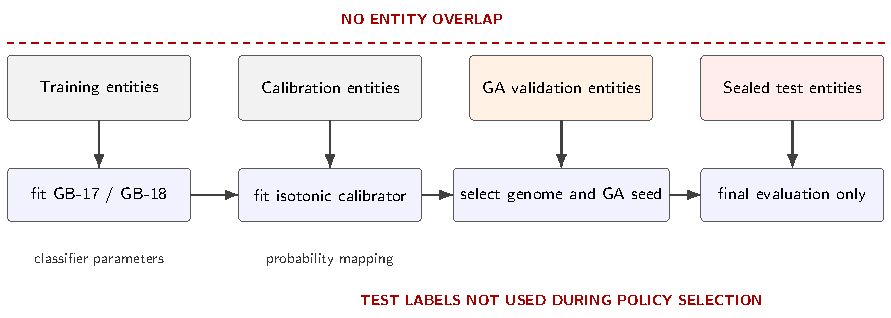
\includegraphics[width=.96\textwidth]{figures/leakage_safe_evaluation.pdf}
\caption{Entity-disjoint training, calibration, policy selection, and sealed evaluation. There is zero entity overlap, and test labels are unavailable before final evaluation.}
\label{fig:evaluation}
\end{figure*}

The baselines isolate two effects. GB-17 versus GB-18 changes only the MiniLM feature and separately fitted calibrator, testing semantic representation under the same fixed policy (RQ1). GB-18 versus GB-18-GA uses the same persisted calibrated GB-18 probabilities, testing only the operating policy (RQ2). For every method and outer seed, complete workflow decisions concatenate exact-tier, model-scored, and blocking-missed rows; the latter enter as positive NO\_MATCH decisions. Precision, recall, F1, FP, FN, REVIEW, and $U$ are independently recomputed from these row-level artifacts and reported as mean $\pm$ sample standard deviation across outer partitions. Outer-partition variation is the only uncertainty summary.

\section{Results}
\subsection{RQ1: Semantic Feature Ablation}
The MiniLM result is mixed rather than uniformly positive. GB-18 exceeds GB-17 for outer seeds 101 and 202, but seed 303 reverses the ordering (Table~\ref{tab:outer}). Consequently, mean fixed-policy F1 is $0.8280\pm0.0223$ for GB-18 and $0.8293\pm0.0278$ for GB-17 (Table~\ref{tab:performance}). Semantic similarity can complement lexical evidence, but one global cosine over concatenated, often incomplete fields does not provide a stable fixed-threshold gain across these partitions.

\begin{table*}[t]
\caption{Authoritative repeated outer-split workflow performance (mean $\pm$ sample SD over three partitions). $U$ is the declared scenario-specific decision objective in (2).}
\label{tab:performance}
\centering
\begin{tabular}{@{}lccccccc@{}}
\toprule
Method & Precision & Recall & F1 & FP & FN & REVIEW & $U$\\
\midrule
GB-17 & .9910\pmv.0051 & .7138\pmv.0431 & .8293\pmv.0278 & 59.0\pmv35.8 & 2265.3\pmv111.7 & 264.7\pmv395.9 & 2409.8\pmv97.2\\
GB-18 & .9940\pmv.0011 & .7100\pmv.0323 & .8280\pmv.0223 & 38.0\pmv7.0 & 2151.0\pmv234.2 & 438.0\pmv406.1 & 2270.8\pmv200.2\\
GB-18-GA & .9889\pmv.0055 & .7615\pmv.0029 & .8604\pmv.0012 & 75.7\pmv38.4 & 1558.0\pmv39.0 & 923.3\pmv151.1 & 1801.7\pmv69.3\\
\bottomrule
\end{tabular}
\end{table*}

\begin{table}[t]
\caption{Authoritative per-partition F1.}
\label{tab:outer}
\centering
\begin{tabular}{@{}crrr@{}}
\toprule
Seed & GB-17 & GB-18 & GB-18-GA\\
\midrule
101 & .8396 & .8410 & .8618\\
202 & .7978 & .8408 & .8600\\
303 & .8504 & .8023 & .8594\\
\bottomrule
\end{tabular}
\end{table}

\subsection{RQ2: Decision-Policy Trade-Off}
GB-18-GA exceeds fixed-policy GB-18 in F1 on every outer test by 0.0208, 0.0192, and 0.0571. Across partitions, mean recall increases from $0.7100$ to $0.7615$, FN decreases by 593.0, and the illustrative objective decreases by 469.1. Because persisted probabilities are unchanged, these differences arise only from reassigning the intermediate score region.

The gains are not free: mean precision decreases from $0.9940$ to $0.9889$, FP rises from 38.0 to 75.7, and REVIEW from 438.0 to 923.3. Thus the GA-selected policy exchanges more false-positive matches and deferred decisions for fewer missed matches; it is an operating-point change rather than universal dominance. The three outer evaluations show the direction and variability of this trade-off but are too few to justify a statistical-significance claim.

\subsection{RQ3: Candidate-Retrieval Ceiling}
Candidate generation reduces the comparison space by 99.5355\%, from 449,149,239 possible cross-platform pairs to 2,086,245 workflow candidates. It covers 25,931 of 29,243 cross-platform positive pairs, so retrieval recall is 88.6742\% and 3,312 true pairs never reach exact or model-scored decisioning. This is a ceiling, not a claimed blocking improvement: no downstream classifier or policy can recover a pair that was not generated. Learned or semantic blocking should therefore be evaluated separately for retrieval gain and computational cost \cite{thirumuruganathan2021deepblocker}.

\section{Failure Analysis and Discussion}
The authoritative workflow decomposition locates two different failure sources. First, candidate generation excludes 3,312 cross-platform positives before classification; these retrieval failures require broader blocking keys or learned candidate generation rather than a new score threshold. Second, among generated test pairs, the GA policy changes FP, FN, and REVIEW counts without changing GB-18 probabilities. Relative to fixed GB-18, it decreases mean FN by 593.0 but adds 37.7 FP and 485.3 REVIEW decisions. This confirms that the gain comes from reallocating uncertain pairs, not from learning a better representation.

The selected trade-off may or may not suit deployment. REVIEW has a lower coefficient than either automatic error in the declared objective, so the GA can defer more cases while reducing missed matches. A workflow with little analyst capacity or very low false-merge tolerance could prefer the fixed policy despite its lower recall. Conversely, a setting that can adjudicate ambiguous pairs may value the additional coverage. Because no reviewers participated, REVIEW counts represent potential workload rather than measured effort or resolution quality.

The mixed GB-17/GB-18 ordering also limits conclusions about semantic evidence. MiniLM cosine is a single compressed view of concatenated name, biography, and location text; missing fields and platform-specific conventions may make its usefulness partition-dependent. Future work should compare field-aware semantic representations and calibration by platform pair. In an Agentic CRM context, the evaluated identity decisions could supply consolidated records upstream, but this study provides no evidence about autonomous agents, lead scoring, or customer outcomes.

\section{Limitations and Threats to Validity}
\emph{Internal validity:} entities, not pairs, are assigned to roles, cross-role pairs are dropped, and the access audit records no test-label request before final evaluation. Nevertheless, source labels may be noisy and are not independently adjudicated. The package hashes the cached 17-feature and MiniLM artifacts used as inputs, but their upstream feature-generation environment is not separately captured.

\emph{External validity:} evidence comes from one transformed historical corpus, three social platforms, and three outer partitions. No external dataset, language transfer, temporal transfer, or live Agentic CRM task is evaluated. The unknown formal dataset license and absent ethics documentation constrain release to code, configuration, hashes, and aggregates unless permission is obtained.

\emph{Construct validity:} $U$ is a declared scenario-specific objective based on engineering assumptions, not an economic, CRM, business, or measured operational cost. REVIEW is an offline decision, not observed analyst effort, agreement, or accuracy. Pair/workflow metrics do not evaluate final entity clusters, CRM outcomes, privacy protection, or lead scoring. Candidate recall bounds the meaning of downstream recall.

\emph{Conclusion validity:} three outer runs provide limited evidence. GA increases FP and REVIEW while improving recall and F1, and no resampling-based interval or human-review study is available. The MiniLM effect is mixed. These constraints preclude statistical-significance, universal-superiority, or cross-corpus generalization claims.

\section{Conclusion}
This study examined how a cross-platform profile matcher should convert calibrated pair evidence into operational decisions. Two entity-disjoint classifier variants isolated one MiniLM feature, after which a GA selected a four-parameter MATCH/REVIEW/NO\_MATCH policy over frozen calibrated GB-18 probabilities. Across three outer evaluations, the selected policy raised mean recall from $0.7100$ to $0.7615$ and mean F1 from $0.8280$ to $0.8604$, while decreasing precision and increasing false-positive and REVIEW counts. The semantic feature alone did not improve the fixed policy consistently. The strongest system limitation occurs before scoring: candidate generation misses 3,312 of 29,243 cross-platform positives. Future work should jointly evaluate improved retrieval, external contemporary corpora, pre-specified decision objectives, and actual human review before assessing downstream Agentic CRM effects.

\bibliographystyle{IEEEtran}
\bibliography{references}
\end{document}
